\question{Интегралы, не зависящие от пути интегрирования. Теорема о независимости интеграла от пути, равносильность I,II,III утверждений.}

Пусть на \(\breve{AB} \in D\) определен \(I = \int_{AB} P \dd x + Q \dd y\),
тогда

\begin{definition}
  Интеграл \(I\) называется независящим от пути интегрирования (далее НЗП), если

  \begin{align*}
    \forall M, N \in D \colon
    \int_{AMB} P\dd x + Q \dd y = \int_{ANB} P\dd x + Q \dd y 
  \end{align*}
\end{definition}

\begin{theorem}\label{path-ind-cr}
  Следующие утверждения равносильны:
  \begin{enumerate}[label = \Roman*.]
    \item \(\int_{AB} P \dd x + Q \dd y\) не зависит от пути.
    \item \(\oint_{K} P \dd x + Q \dd y = 0\).
    \item \(P'_{y} = Q'_{x}\) (везде в области \(D\)).
    \item \(\exists \Phi(x, y) \colon \dd \Phi = P \dd x + Q \dd y\).
  \end{enumerate}
\end{theorem}
\begin{proof}
  \(I \implies II\) (НЗП \(\implies \oint = 0\))

  Если интеграл не зависит от пути, то по определению:

  \begin{align*}
    \int_{AMB} = \int_{ANB}
    \implies \int_{AMB} - \int_{ANB} = 0
    \implies \int_{AMB} + \int_{BNA} = 0
    \implies \oint_{K} = 0
  \end{align*}
\end{proof}
\begin{proof}
  \(I \impliedby II\) (НЗП \(\impliedby \oint = 0\))

  Пусть в области \(D\) есть некоторые точки \(M\) и \(N\), тогда интеграл по
  контуру можно представить в виде:

  \begin{align*}
    \oint_{K} = 0
    \implies \int_{AMB} + \int_{BNA} = 0
    \implies \int_{AMB} - \int_{ANB} = 0
    \implies \int_{AMB} = \int_{ANB}
  \end{align*}

  Т.к. точки \(M\) и \(N\) выбраны произвольно \(\in D\), то это выполняется для
  любых точек \(M\), \(N \implies\) интеграл не зависит от пути по определению.
\end{proof}
\begin{proof}
  \(II \implies III\) (\(\oint = 0 \implies P'_{y} = Q'_{x}\))

  От противного: пусть

  \begin{align*}
    \exists M (x_{0}, y_{0}) \in D \colon P'_{y} \neq Q'_{x}
    \implies Q'_{x} - P'_{y} > 0
  \end{align*}

  Знак больше выбран для определенности, можно и рассмотреть и с минусом:
  доказательство будет аналогичным.

  Окружим точку \(M(x_{0}, y_{0})\) окрестностью \(u_{\epsilon}(M_{0})\).
  Применим формулу Грина для \(K = \Gamma_{u}\):

  \begin{align*}
    \oint_{K} P \dd x + Q \dd y
    = \iint_{u(M_{0})} (Q'_{x} - P'_{y}) \dd x \dd y \\
    Q'_{x} - P'_{y} > 0
      \implies \exists \delta \in \RR^{+} \colon Q'_{x} - P'_{y} > \delta > 0 \\
    \iint_{u(M_{0})} (Q'_{x} - P'_{y}) \dd x \dd y
      > \iint_{u(M_{0})} \delta \dd x \dd y
      = \delta S(u(M_{0})) > 0
  \end{align*}

  Получаем, что \(\oint_{K} P \dd x + Q \dd y > 0\). Противоречие.
\end{proof}
\begin{proof}
  \(II \impliedby III\) (\(\oint = 0 \impliedby P'_{y} = Q'_{x}\))

  Применяем формулу Грина:

  \begin{align*}
    P'_{y} = Q'_{x} \implies Q'_{x} - P'_{y} = 0 \\
      \int_{D} (Q'_{x} - P'_{y}) \dd x \dd y
      = 0
      = \oint_{K = \Gamma_{D}} P \dd x + Q \dd y
  \end{align*}
\end{proof}
\begin{proof}
  \(I \implies IV\) (НЗП \(\implies \exists \Phi(x, y)\))

  Рассмотрим интеграл \(\int_{AB} P \dd x + Q \dd y\).
  Заменим точку \(B\) на 'плавающую' точку \(M(x, y)\). Получим:

  \begin{align*}
    \Phi(x, y) = \int_{AM} P \dd x + Q \dd y \\
    \dd \Phi
    = \frac{\partial \Phi}{\partial x} \dd x
      + \frac{\partial \Phi}{\partial y} \dd y
    \label{eq:phi-diff}\tag{1}
  \end{align*}

  Покажем, что \(\displaystyle \frac{\partial \Phi}{\partial x} = P(x, y)\).
  Рассмотрим частное приращение функции \(\Phi(x, y)\) по \(x\):

  \begin{align*}
    \Delta_{x} \Phi
    = \Phi(x + \Delta x, y) - \Phi(x, y)
    = \int_{AM_{1}} - \int_{AM}
    = \int_{MM_{1}}
    = \int_{MM_{1}} P \dd x + Q \dd y
  \end{align*}

  где точка \(M_{1}\) имеет координаты \((x + \Delta x, y)\). Т.к. интеграл не
  зависит от пути, то выберем удобный путь интегрирования
  \(y = const \implies \dd y = 0\):

  \begin{align*}
    \int_{MM_{1}} P \dd x + Q \dd y
    = \int_{MM_{1}} P \dd x
  \end{align*}

  Воспользуемся т. Лагранжа о среднем(\ref{L-mid-int}):

  \begin{align*}
    \exists \xi \in (x, x + \Delta x) \colon 
      \int_{MM_{1}} P \dd x = P(\xi, y) \Delta x    
  \end{align*}

  В итоге получаем, что
  
  \begin{align*}
    \Phi(x + \Delta x, y) - \Phi(x, y) = P(\xi, y) \Delta x
  \end{align*}

  Подставим это в определение частной производной  для
  \(\displaystyle \frac{\partial \Phi}{\partial x}\):

  \begin{align*}
    \frac{\partial \Phi}{\partial x}
    = \lim_{\Delta x \to 0}
      \frac{\Phi(x + \Delta x, y) - \Phi(x, y)}{\Delta x}
    = \lim_{\Delta x \to 0} P(\xi, y)
    = \begin{bmatrix}
      \begin{rcases}
        \Delta x \to 0 \\
        \xi \in (x, x + \Delta x)
      \end{rcases}
      \implies \xi \to x
    \end{bmatrix}
    = P(x, y)
  \end{align*}

  Аналогично можно показать, что
  \(\displaystyle \frac{\partial \Phi}{\partial y} = Q(x, y)\).
  Подставляя полученные выражения в \eqref{eq:phi-diff} получаем искомое
  равенство.
\end{proof}
\begin{proof}
  \(III \impliedby IV\) (\(P'_{y} = Q'_{x} \impliedby \exists \Phi(x, y)\))

  Раскроем дифференциал функции \(\Phi(x, y)\) по определению:

  \begin{align*}
    P \dd x + Q \dd y
    = \dd \Phi
    = \frac{\partial \Phi}{\partial x} \dd x
      + \frac{\partial \Phi}{\partial y} \dd y
  \end{align*}

  Далее возьмем частные производные \(P'_{y}\) и \(Q'_{x}\):

  \begin{align*}
    \frac{\partial P}{\partial y}
      = \frac{\partial^2 \Phi}{\partial x \partial y} 
      = \frac{\partial Q}{\partial x}
  \end{align*}
\end{proof}

\begin{remark}
  Функция \(\Phi(x, y)\) называется потенциалом, либо первообразной для
  подынтегрального выражения.
\end{remark}

\begin{twocolumns}
  \begin{figure}[H]
  \centering

  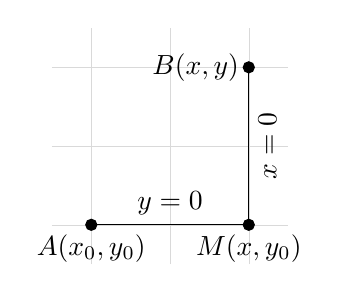
\begin{tikzpicture}
    \draw[very thin, gray!30, step = 1cm] (0.5, 0.5) grid (3.5, 3.5);
    
    \draw[fill = black] (1, 1) circle (2pt);
    \draw node[below] at (1, 1) {\(A(x_{0}, y_{0})\)};
  
    \draw[fill = black] (3, 1) circle (2pt);
    \draw node[below] at (3, 1) {\(M(x, y_{0})\)};
  
    \draw[fill = black] (3, 3) circle (2pt);
    \draw node[left] at (3, 3) {\(B(x, y)\)};
  
    \draw (1, 1) -- (3, 1)
      node[midway, above] {\(\dd y = 0\)};
    \draw (3, 3) -- (3, 1)
      node[midway, below, sloped, rotate = 180] {\(\dd x = 0\)};
  \end{tikzpicture}  
\end{figure}
  \columnbreak

  \begin{remark}
    Если интеграл не зависит от пути, то частно бывает удобно рассмотреть путь
    \(A(x_{0}, y_{0}) \to M(x, y_{0}) \to B(x, y)\). При таким подходе интеграл
    разбивается на два, причем в каждом из них половина обнуляется (т.к.
    \(\dd x = 0\) либо \(\dd y = 0\)).
  \end{remark}
\end{twocolumns}



